% !TEX TS-program = xelatex
% !TEX encoding = UTF-8 Unicode
% !Mode:: "TeX:UTF-8"

\documentclass{resume}
\usepackage{zh_CN-Adobefonts_external} % Simplified Chinese Support using external fonts (./fonts/zh_CN-Adobe/)
%\usepackage{zh_CN-Adobefonts_internal} % Simplified Chinese Support using system fonts
\usepackage{linespacing_fix} % disable extra space before next section
\usepackage{cite}
\usepackage{tabu}
\usepackage{multirow}
\usepackage{graphicx}

\begin{document}
\pagenumbering{gobble} % suppress displaying page number

  \begin{tabu}{ c l r }
   \multirow{5}{1in}{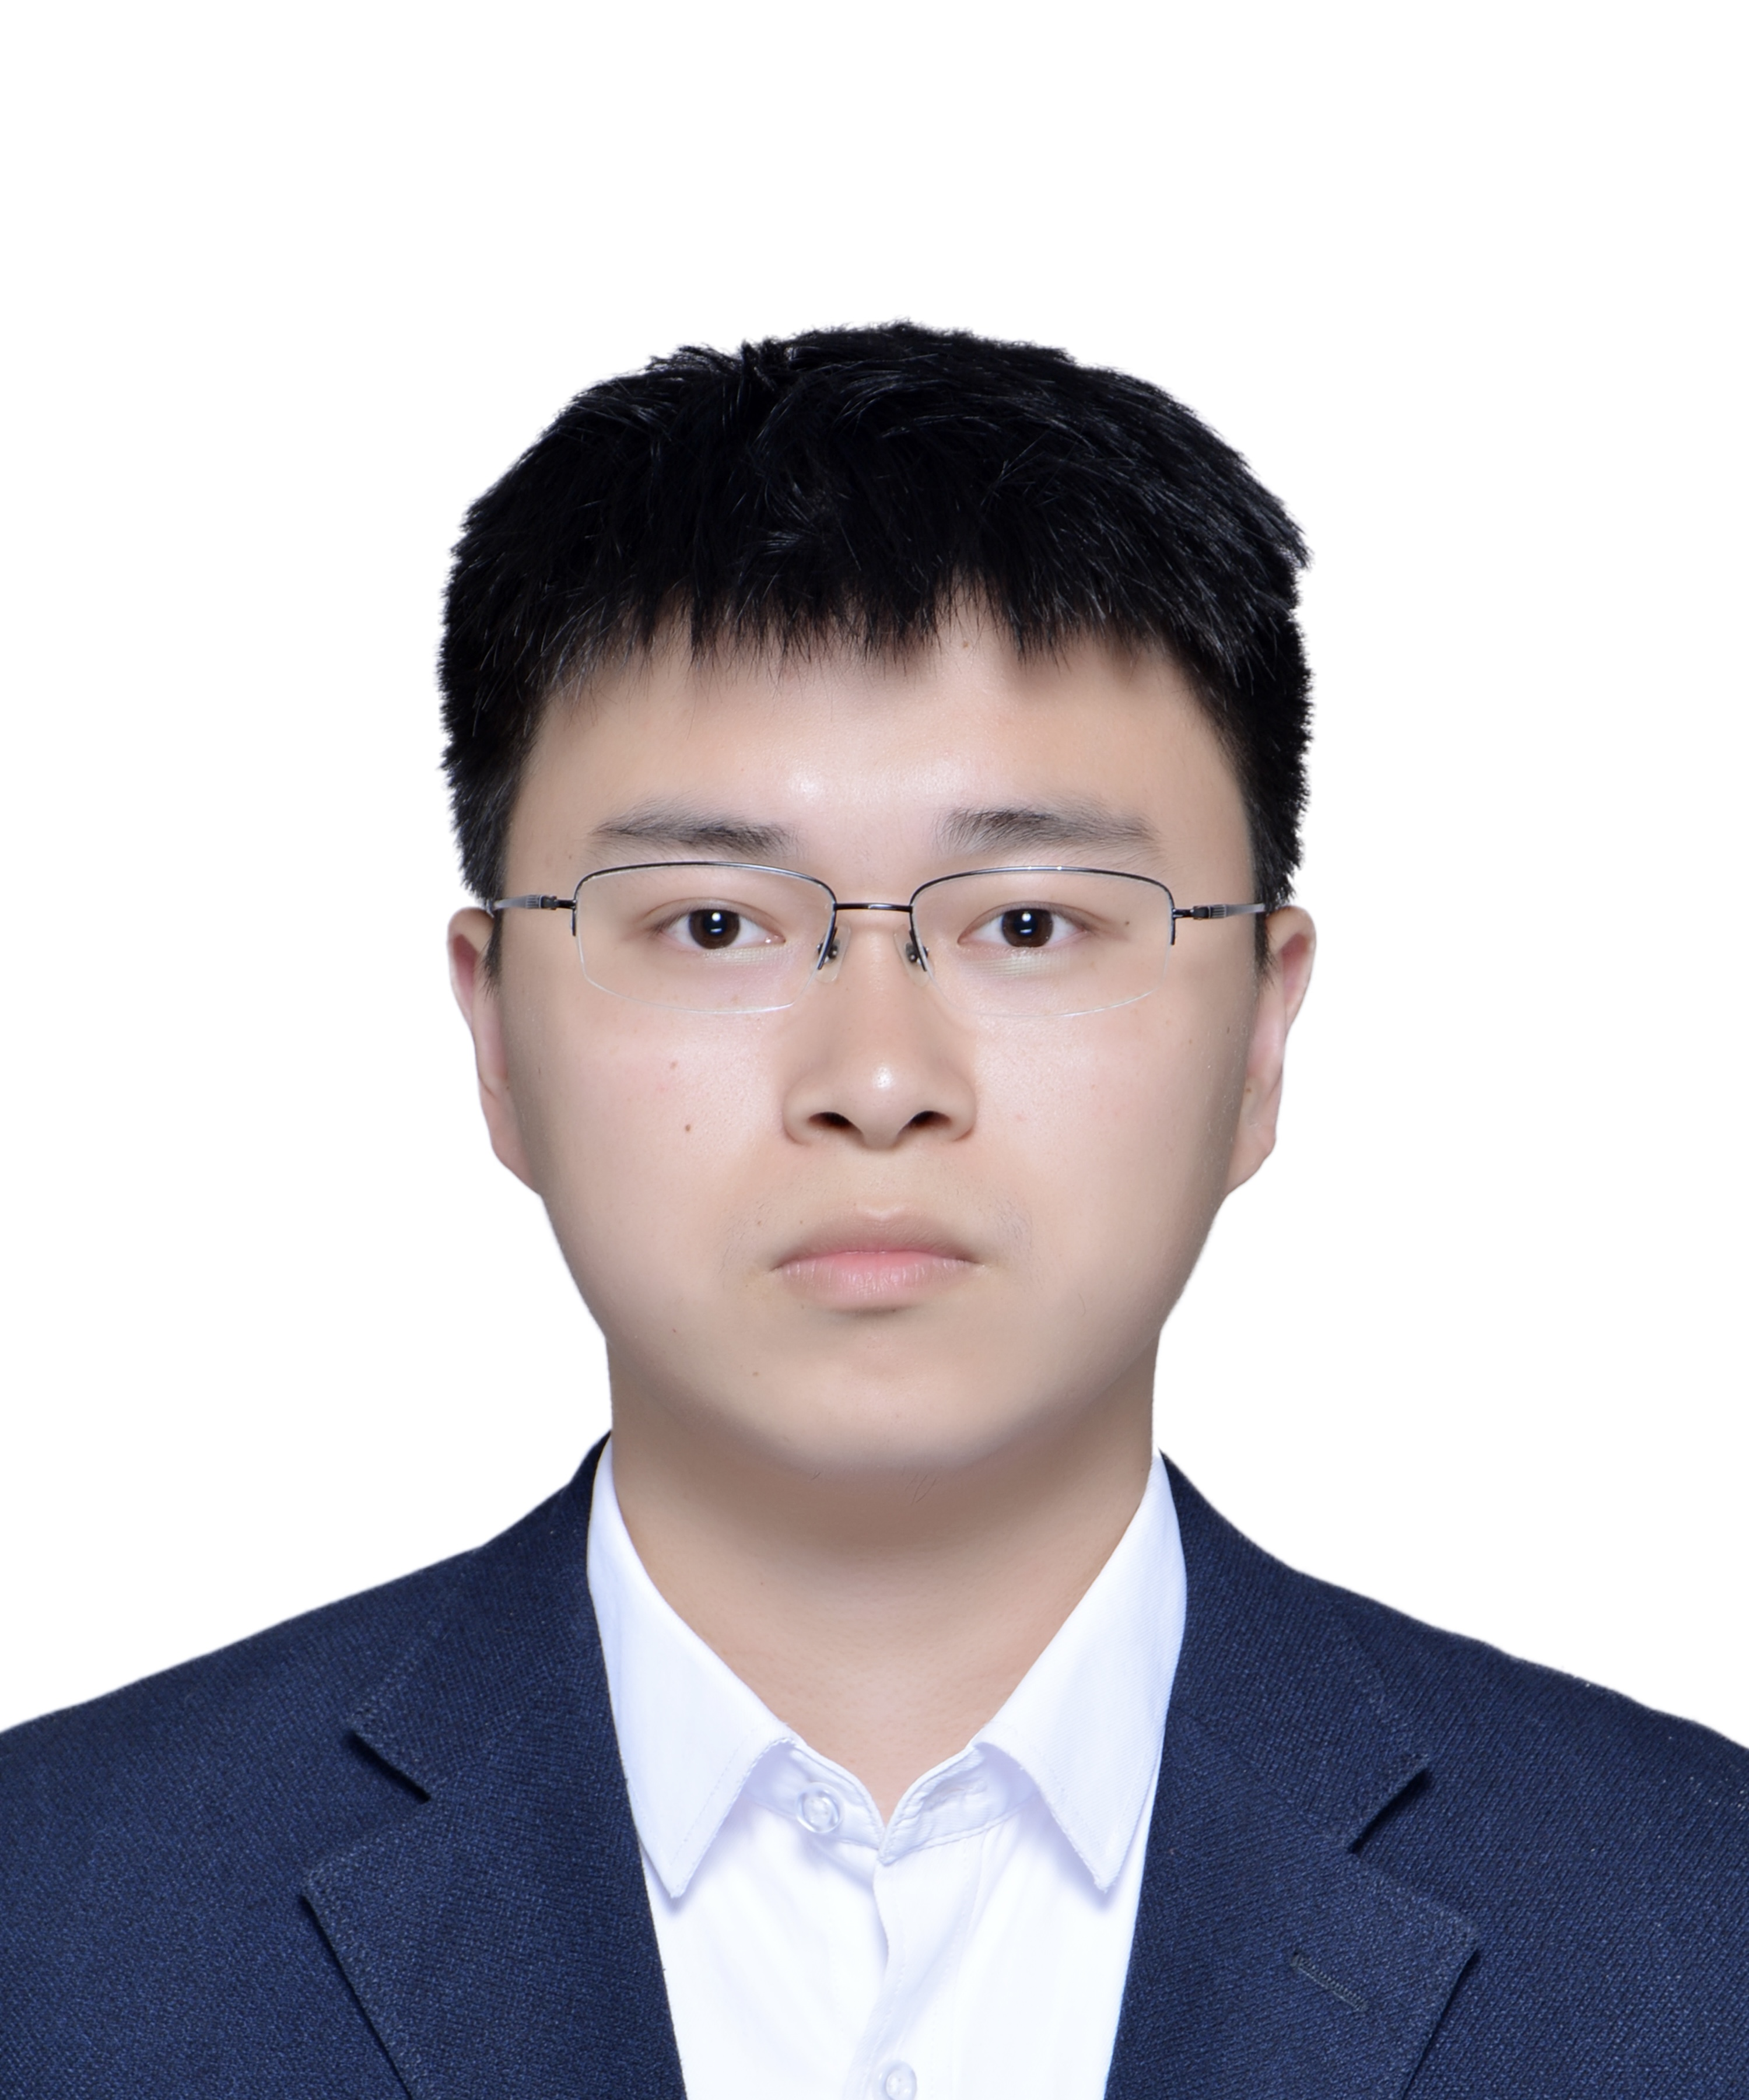
\includegraphics[width=0.88in]{avatar.jpg}} \\ 
    & \Large{\songti{吴亚戌}}\\
    & \email{wuyaxu.info@gmail.com}\\
    & \phone{(+86) 139-7230-6166} \\
    & \github[github.com/wuyaxv]{https://github.com/wuyaxv} \\
    & \faLink{wuyaxv.github.io}
  \end{tabu}
\\[2pt]

%\basicInfo{
%  \email{wuyaxu.info@gmail.com} \textperiodcentered\ 
%  \phone{(+86) 139-7230-6166} \textperiodcentered\ 
%  \hyperlink{https://wuyaxv.github.io}{wuyaxv.github.io}
%  }

 
\section{\faGraduationCap\  教育背景}
\datedsubsection{\textbf{重庆邮电大学, 网络空间安全与信息法学院}, 重庆}{2021年9月 -- 至今}
\textit{学士在读}\ 信息安全,预计 2024 年 6 月毕业
\datedsubsection{\textbf{重庆邮电大学, 先进制造工程学院}, 重庆}{2020年9月 -- 2021年6月}
智能制造专业

\section{\faUsers\ 项目经历}
\datedsubsection{\textbf{基于5G \& NTN输电线路监控系统}}{2021年9月 -- 2022年5月}
\role{市场调研与前端开发}{大学生创新创业训练项目,指导老师:彭大芹}
\begin{itemize}
  \item 负责搜集近十年国内外架空输电线路建设里程数据;
  \item 研究国家与行业标准,整理和分析国家统计局及相关投资机构的行业发展报告;
  \item 计算行业市场规模,并独立完成商业计划书中市场研究报告的撰写;
  \item 参与了检测状态页面原型的开发和状态数据格式的设计,编写脚本对数据进行格式化处理
\end{itemize}
\datedsubsection{\textbf{基于Wazuh的SIEM平台开发}}{2022年9月 -- 2023年5月}
\role{KVM, QEMU, libvirt, Python}{大学生科研训练计划项目,指导老师:程克非}
本人负责项目的虚拟仿真环境的搭建, \href{https://github.com/wuyaxv/ShortCuts/wazuh}{github.com/wuyaxv/ShortCuts/wazuh}
\begin{itemize}
  \item 提出搭建IaaS平台并使用KVM技术开发SIEM仿真环境等方案,被小组采纳;
  \item 基于virt-tools开发了一系列bash脚本用于虚拟机迁移环境的快速部署;
  \item 使用libvirt开发了项目的V2V和P2V功能,实现了一个可用原型
\end{itemize}

\datedsubsection{\textbf{基于WireGuard的P2P Mesh组网应用}}{2023 年12月 -- 至今}
\role{WireGuard, C, Python}{个人项目}
一个基于WireGuard的P2P组网系统,\href{https://github.com/wuyaxv/grad_proj}{github.com/wuyaxv/grad\_proj}
\begin{itemize}
  \item 实现Overlay网络以解决星型组网造成大量不必要服务器流量的问题;
  \item 探究通过Mesh组网降低上行带宽不足之影响以提高P2P网络传输效率;
  \item 高联通性的内网穿透方案
\end{itemize}

% Reference Test
%\datedsubsection{\textbf{Paper Title\cite{zaharia2012resilient}}}{May. 2015}
%An xxx optimized for xxx\cite{verma2015large}
%\begin{itemize}
%  \item main contribution
%\end{itemize}

\section{\faCogs\ 个人技能}
% increase linespacing [parsep=0.5ex]
\begin{itemize}[parsep=0.5ex]
  \item 编程语言: C / Python / C++ / Bash / HTML / MySQL / SQLite / GNU as / nasm 
  \item 其他能力: Makefile / \LaTeX / QEMU / Ghidra / x86 binary exploitation
  \item 语言能力: 英语阅读和听力(熟练),英语写作(较好);CET-4(613分), CET-6(562分)
\end{itemize}

\section{\faTrophy\ 获奖情况}
\datedline{第十五届全国大学生数学竞赛 \textit{一等奖}}{}
\datedline{2023年全国大学生英语竞赛 \textit{一等奖}}{}
\datedline{2021年全国大学生英语竞赛 \textit{三等奖}}{}
\datedline{第八届“美亚杯”电子数据取证大赛 \textit{二等奖}}{}
\datedline{第四届西电“长安杯”电子数据取证大赛 \textit{二等奖}}{}
\datedline{第十四届蓝桥杯(本科软件类B组)\textit{市三等奖}}{}
\datedline{2022年学业 \textit{三等奖学金}}
\datedline{2023年学业 \textit{二等奖学金}}

%% Reference
%\newpage
%\bibliographystyle{IEEETran}
%\bibliography{mycite}
\end{document}
